% Shared preamble for CS 377 worksheets.
%
% Usage: a worksheet begins with % Shared preamble for CS 377 worksheets.
%
% Usage: a worksheet begins with % Shared preamble for CS 377 worksheets.
%
% Usage: a worksheet begins with \input{00-template.tex}, sets its metadata with
% \wscourse / \wstitle, then opens \begin{document} and calls
% \wsheader (group version) or \wsheaderindividual (individual version).
%
% Build with build.sh (pdflatex).

\documentclass[11pt]{article}

\usepackage[T1]{fontenc}
\usepackage[utf8]{inputenc}
\usepackage{lmodern}
\usepackage[margin=0.9in, top=0.75in, bottom=0.75in]{geometry}
\usepackage{microtype}
\usepackage{array}
\usepackage{tabularx}
\usepackage{calc}
\usepackage{enumitem}
\usepackage{forloop}

\setlength{\parindent}{0pt}
\setlength{\parskip}{0.5\baselineskip}
\pagestyle{empty}
\raggedbottom

% Vertically center the contents of every X column, so that short entries sit in
% the middle of a tall ruled row rather than clinging to its top edge.
\renewcommand{\tabularxcolumn}[1]{m{#1}}

% ---------------------------------------------------------------------------
% Metadata
% ---------------------------------------------------------------------------
\newcommand{\wscourseval}{CS 377}
\newcommand{\wstitleval}{Worksheet}

\newcommand{\wscourse}[1]{\renewcommand{\wscourseval}{#1}}
\newcommand{\wstitle}[1]{\renewcommand{\wstitleval}{#1}}

% Section meeting times offered in the current term, one per column of the
% "circle one" row. Fall 2026 has two sections. To add or drop one, edit both
% \wssections and \wssectioncount.
\newcommand{\wssections}{\wssectiontime{12:30pm} & \wssectiontime{2:00pm}}
\newcommand{\wssectioncount}{2}

% ---------------------------------------------------------------------------
% Header pieces
% ---------------------------------------------------------------------------

% Course number, small and right-aligned above the title.
\newcommand{\wscourseline}{%
  {\raggedleft\small\wscourseval\par}%
  \vspace{0.4\baselineskip}%
}

\newcommand{\wsbigtitle}{%
  {\fontsize{26}{30}\selectfont\bfseries\wstitleval\par}%
  \vspace{0.4\baselineskip}%
}

% Four ruled boxes (2x2) for group members to sign in.
\newcommand{\wsmembertable}{%
  \begin{tabularx}{\textwidth}{|X|X|}
    \hline
    \rule{0pt}{2.4\baselineskip} & \\
    \hline
    \rule{0pt}{2.4\baselineskip} & \\
    \hline
  \end{tabularx}%
}

% Single ruled box for a name.
\newcommand{\wsnametable}{%
  \begin{tabularx}{\textwidth}{|>{\raggedleft\arraybackslash\bfseries}m{1.4in}|X|}
    \hline
    Your Name & \rule{0pt}{2.4\baselineskip} \\
    \hline
  \end{tabularx}%
}

% A cell of fixed height whose contents are vertically centered.
%
% An m-column is not enough on its own: it centers the cell's *box*, which for a
% multi-line paragraph leaves the text riding high against the top rule. Giving
% every cell in the row an explicit equal-height parbox with [c] inner alignment
% centers the text itself, whether it is one line or two.
\newcommand{\wsvcell}[2]{\parbox[c][#1][c]{\linewidth}{#2}}

% "Section (circle one)" row with one column per meeting time. The row height is
% measured once at the surrounding font size, so that the \small label and the
% normal-size times agree on how tall the row is.
\newlength{\wssectionrowht}
\newcommand{\wssectiontime}[1]{\wsvcell{\wssectionrowht}{\centering #1}}
\newcommand{\wssectiontable}{%
  \setlength{\wssectionrowht}{2.6\baselineskip}%
  \begin{tabularx}{\textwidth}{|>{\bfseries\small}m{1.1in}|*{\wssectioncount}{X|}}
    \hline
    \wsvcell{\wssectionrowht}{\raggedleft Section\newline(circle one)} & \wssections \\
    \hline
  \end{tabularx}%
}

% Group worksheet header: course, title, group members, section.
\newcommand{\wsheader}{%
  \wscourseline
  \wsbigtitle
  Group members:\par
  \vspace{0.2\baselineskip}
  \wsmembertable
  \vspace{0.6\baselineskip}
  \wssectiontable
  \vspace{0.4\baselineskip}
}

% Individual worksheet header: course/date, title, name, section.
\newcommand{\wsheaderindividual}{%
  \wscourseline
  \wsbigtitle
  \wsnametable
  \vspace{0.6\baselineskip}
  \wssectiontable
  \vspace{0.4\baselineskip}
}

% ---------------------------------------------------------------------------
% Questions
% ---------------------------------------------------------------------------
\newcounter{wsquestion}

% \wsquestion{prompt}{writing space} -- auto-numbered prompt followed by blank
% space for students to write in.
\newcommand{\wsquestion}[2]{%
  \stepcounter{wsquestion}%
  \par\noindent(\thewsquestion)~#1\par
  \vspace{#2}%
}

% Prompt with no trailing space, for when a table or list follows.
\newcommand{\wsprompt}[1]{%
  \stepcounter{wsquestion}%
  \par\noindent(\thewsquestion)~#1\par
}

% Worksheet tables: a header row of italic headings over a stack of tall blank
% rows for students to write in.
%
% \wsgridtable{left heading}{right heading}{number of rows}{row height}
% \wsgridtablethree{left}{middle}{right}{number of rows}{row height}
%
% The blank rows are accumulated into \wsrowsbody *before* the tabularx is
% opened. Running the loop inside the table instead leaves a stray extra row,
% because the loop's own machinery counts as the start of one.
\newcounter{wsrow}
\newcounter{wscol}
\makeatletter
\newcommand{\wsrowsbody}{}
% \wsbuildrows{number of rows}{row height}{number of columns}
\newcommand{\wsbuildrows}[3]{%
  \gdef\wsrowsbody{}%
  \forloop{wsrow}{0}{\value{wsrow} < #1}{%
    \g@addto@macro\wsrowsbody{\rule[-0.5\baselineskip]{0pt}{#2}}%
    \forloop{wscol}{1}{\value{wscol} < #3}{%
      \g@addto@macro\wsrowsbody{&}%
    }%
    \g@addto@macro\wsrowsbody{\\ \hline}%
  }%
}
\makeatother

% Each heading gets an equal-height centered cell, so that the headings line up
% with each other and sit centered in the heading row rather than against its
% top rule.
\newlength{\wsheadht}
\newcommand{\wshead}[1]{\wsvcell{\wsheadht}{\itshape #1}}

\newcommand{\wsgridtable}[4]{%
  \wsbuildrows{#3}{#4}{2}%
  \setlength{\wsheadht}{1.6\baselineskip}%
  \begin{tabularx}{\textwidth}{|X|X|}
    \hline
    \wshead{#1} & \wshead{#2} \\
    \hline
    \wsrowsbody
  \end{tabularx}%
}

\newcommand{\wsgridtablethree}[5]{%
  \wsbuildrows{#4}{#5}{3}%
  \setlength{\wsheadht}{1.6\baselineskip}%
  \begin{tabularx}{\textwidth}{|X|X|X|}
    \hline
    \wshead{#1} & \wshead{#2} & \wshead{#3} \\
    \hline
    \wsrowsbody
  \end{tabularx}%
}
, sets its metadata with
% \wscourse / \wstitle, then opens \begin{document} and calls
% \wsheader (group version) or \wsheaderindividual (individual version).
%
% Build with build.sh (pdflatex).

\documentclass[11pt]{article}

\usepackage[T1]{fontenc}
\usepackage[utf8]{inputenc}
\usepackage{lmodern}
\usepackage[margin=0.9in, top=0.75in, bottom=0.75in]{geometry}
\usepackage{microtype}
\usepackage{array}
\usepackage{tabularx}
\usepackage{calc}
\usepackage{enumitem}
\usepackage{forloop}

\setlength{\parindent}{0pt}
\setlength{\parskip}{0.5\baselineskip}
\pagestyle{empty}
\raggedbottom

% Vertically center the contents of every X column, so that short entries sit in
% the middle of a tall ruled row rather than clinging to its top edge.
\renewcommand{\tabularxcolumn}[1]{m{#1}}

% ---------------------------------------------------------------------------
% Metadata
% ---------------------------------------------------------------------------
\newcommand{\wscourseval}{CS 377}
\newcommand{\wstitleval}{Worksheet}

\newcommand{\wscourse}[1]{\renewcommand{\wscourseval}{#1}}
\newcommand{\wstitle}[1]{\renewcommand{\wstitleval}{#1}}

% Section meeting times offered in the current term, one per column of the
% "circle one" row. Fall 2026 has two sections. To add or drop one, edit both
% \wssections and \wssectioncount.
\newcommand{\wssections}{\wssectiontime{12:30pm} & \wssectiontime{2:00pm}}
\newcommand{\wssectioncount}{2}

% ---------------------------------------------------------------------------
% Header pieces
% ---------------------------------------------------------------------------

% Course number, small and right-aligned above the title.
\newcommand{\wscourseline}{%
  {\raggedleft\small\wscourseval\par}%
  \vspace{0.4\baselineskip}%
}

\newcommand{\wsbigtitle}{%
  {\fontsize{26}{30}\selectfont\bfseries\wstitleval\par}%
  \vspace{0.4\baselineskip}%
}

% Four ruled boxes (2x2) for group members to sign in.
\newcommand{\wsmembertable}{%
  \begin{tabularx}{\textwidth}{|X|X|}
    \hline
    \rule{0pt}{2.4\baselineskip} & \\
    \hline
    \rule{0pt}{2.4\baselineskip} & \\
    \hline
  \end{tabularx}%
}

% Single ruled box for a name.
\newcommand{\wsnametable}{%
  \begin{tabularx}{\textwidth}{|>{\raggedleft\arraybackslash\bfseries}m{1.4in}|X|}
    \hline
    Your Name & \rule{0pt}{2.4\baselineskip} \\
    \hline
  \end{tabularx}%
}

% A cell of fixed height whose contents are vertically centered.
%
% An m-column is not enough on its own: it centers the cell's *box*, which for a
% multi-line paragraph leaves the text riding high against the top rule. Giving
% every cell in the row an explicit equal-height parbox with [c] inner alignment
% centers the text itself, whether it is one line or two.
\newcommand{\wsvcell}[2]{\parbox[c][#1][c]{\linewidth}{#2}}

% "Section (circle one)" row with one column per meeting time. The row height is
% measured once at the surrounding font size, so that the \small label and the
% normal-size times agree on how tall the row is.
\newlength{\wssectionrowht}
\newcommand{\wssectiontime}[1]{\wsvcell{\wssectionrowht}{\centering #1}}
\newcommand{\wssectiontable}{%
  \setlength{\wssectionrowht}{2.6\baselineskip}%
  \begin{tabularx}{\textwidth}{|>{\bfseries\small}m{1.1in}|*{\wssectioncount}{X|}}
    \hline
    \wsvcell{\wssectionrowht}{\raggedleft Section\newline(circle one)} & \wssections \\
    \hline
  \end{tabularx}%
}

% Group worksheet header: course, title, group members, section.
\newcommand{\wsheader}{%
  \wscourseline
  \wsbigtitle
  Group members:\par
  \vspace{0.2\baselineskip}
  \wsmembertable
  \vspace{0.6\baselineskip}
  \wssectiontable
  \vspace{0.4\baselineskip}
}

% Individual worksheet header: course/date, title, name, section.
\newcommand{\wsheaderindividual}{%
  \wscourseline
  \wsbigtitle
  \wsnametable
  \vspace{0.6\baselineskip}
  \wssectiontable
  \vspace{0.4\baselineskip}
}

% ---------------------------------------------------------------------------
% Questions
% ---------------------------------------------------------------------------
\newcounter{wsquestion}

% \wsquestion{prompt}{writing space} -- auto-numbered prompt followed by blank
% space for students to write in.
\newcommand{\wsquestion}[2]{%
  \stepcounter{wsquestion}%
  \par\noindent(\thewsquestion)~#1\par
  \vspace{#2}%
}

% Prompt with no trailing space, for when a table or list follows.
\newcommand{\wsprompt}[1]{%
  \stepcounter{wsquestion}%
  \par\noindent(\thewsquestion)~#1\par
}

% Worksheet tables: a header row of italic headings over a stack of tall blank
% rows for students to write in.
%
% \wsgridtable{left heading}{right heading}{number of rows}{row height}
% \wsgridtablethree{left}{middle}{right}{number of rows}{row height}
%
% The blank rows are accumulated into \wsrowsbody *before* the tabularx is
% opened. Running the loop inside the table instead leaves a stray extra row,
% because the loop's own machinery counts as the start of one.
\newcounter{wsrow}
\newcounter{wscol}
\makeatletter
\newcommand{\wsrowsbody}{}
% \wsbuildrows{number of rows}{row height}{number of columns}
\newcommand{\wsbuildrows}[3]{%
  \gdef\wsrowsbody{}%
  \forloop{wsrow}{0}{\value{wsrow} < #1}{%
    \g@addto@macro\wsrowsbody{\rule[-0.5\baselineskip]{0pt}{#2}}%
    \forloop{wscol}{1}{\value{wscol} < #3}{%
      \g@addto@macro\wsrowsbody{&}%
    }%
    \g@addto@macro\wsrowsbody{\\ \hline}%
  }%
}
\makeatother

% Each heading gets an equal-height centered cell, so that the headings line up
% with each other and sit centered in the heading row rather than against its
% top rule.
\newlength{\wsheadht}
\newcommand{\wshead}[1]{\wsvcell{\wsheadht}{\itshape #1}}

\newcommand{\wsgridtable}[4]{%
  \wsbuildrows{#3}{#4}{2}%
  \setlength{\wsheadht}{1.6\baselineskip}%
  \begin{tabularx}{\textwidth}{|X|X|}
    \hline
    \wshead{#1} & \wshead{#2} \\
    \hline
    \wsrowsbody
  \end{tabularx}%
}

\newcommand{\wsgridtablethree}[5]{%
  \wsbuildrows{#4}{#5}{3}%
  \setlength{\wsheadht}{1.6\baselineskip}%
  \begin{tabularx}{\textwidth}{|X|X|X|}
    \hline
    \wshead{#1} & \wshead{#2} & \wshead{#3} \\
    \hline
    \wsrowsbody
  \end{tabularx}%
}
, sets its metadata with
% \wscourse / \wstitle, then opens \begin{document} and calls
% \wsheader (group version) or \wsheaderindividual (individual version).
%
% Build with build.sh (pdflatex).

\documentclass[11pt]{article}

\usepackage[T1]{fontenc}
\usepackage[utf8]{inputenc}
\usepackage{lmodern}
\usepackage[margin=0.9in, top=0.75in, bottom=0.75in]{geometry}
\usepackage{microtype}
\usepackage{array}
\usepackage{tabularx}
\usepackage{calc}
\usepackage{enumitem}
\usepackage{forloop}

\setlength{\parindent}{0pt}
\setlength{\parskip}{0.5\baselineskip}
\pagestyle{empty}
\raggedbottom

% Vertically center the contents of every X column, so that short entries sit in
% the middle of a tall ruled row rather than clinging to its top edge.
\renewcommand{\tabularxcolumn}[1]{m{#1}}

% ---------------------------------------------------------------------------
% Metadata
% ---------------------------------------------------------------------------
\newcommand{\wscourseval}{CS 377}
\newcommand{\wstitleval}{Worksheet}

\newcommand{\wscourse}[1]{\renewcommand{\wscourseval}{#1}}
\newcommand{\wstitle}[1]{\renewcommand{\wstitleval}{#1}}

% Section meeting times offered in the current term, one per column of the
% "circle one" row. Fall 2026 has two sections. To add or drop one, edit both
% \wssections and \wssectioncount.
\newcommand{\wssections}{\wssectiontime{12:30pm} & \wssectiontime{2:00pm}}
\newcommand{\wssectioncount}{2}

% ---------------------------------------------------------------------------
% Header pieces
% ---------------------------------------------------------------------------

% Course number, small and right-aligned above the title.
\newcommand{\wscourseline}{%
  {\raggedleft\small\wscourseval\par}%
  \vspace{0.4\baselineskip}%
}

\newcommand{\wsbigtitle}{%
  {\fontsize{26}{30}\selectfont\bfseries\wstitleval\par}%
  \vspace{0.4\baselineskip}%
}

% Four ruled boxes (2x2) for group members to sign in.
\newcommand{\wsmembertable}{%
  \begin{tabularx}{\textwidth}{|X|X|}
    \hline
    \rule{0pt}{2.4\baselineskip} & \\
    \hline
    \rule{0pt}{2.4\baselineskip} & \\
    \hline
  \end{tabularx}%
}

% Single ruled box for a name.
\newcommand{\wsnametable}{%
  \begin{tabularx}{\textwidth}{|>{\raggedleft\arraybackslash\bfseries}m{1.4in}|X|}
    \hline
    Your Name & \rule{0pt}{2.4\baselineskip} \\
    \hline
  \end{tabularx}%
}

% A cell of fixed height whose contents are vertically centered.
%
% An m-column is not enough on its own: it centers the cell's *box*, which for a
% multi-line paragraph leaves the text riding high against the top rule. Giving
% every cell in the row an explicit equal-height parbox with [c] inner alignment
% centers the text itself, whether it is one line or two.
\newcommand{\wsvcell}[2]{\parbox[c][#1][c]{\linewidth}{#2}}

% "Section (circle one)" row with one column per meeting time. The row height is
% measured once at the surrounding font size, so that the \small label and the
% normal-size times agree on how tall the row is.
\newlength{\wssectionrowht}
\newcommand{\wssectiontime}[1]{\wsvcell{\wssectionrowht}{\centering #1}}
\newcommand{\wssectiontable}{%
  \setlength{\wssectionrowht}{2.6\baselineskip}%
  \begin{tabularx}{\textwidth}{|>{\bfseries\small}m{1.1in}|*{\wssectioncount}{X|}}
    \hline
    \wsvcell{\wssectionrowht}{\raggedleft Section\newline(circle one)} & \wssections \\
    \hline
  \end{tabularx}%
}

% Group worksheet header: course, title, group members, section.
\newcommand{\wsheader}{%
  \wscourseline
  \wsbigtitle
  Group members:\par
  \vspace{0.2\baselineskip}
  \wsmembertable
  \vspace{0.6\baselineskip}
  \wssectiontable
  \vspace{0.4\baselineskip}
}

% Individual worksheet header: course/date, title, name, section.
\newcommand{\wsheaderindividual}{%
  \wscourseline
  \wsbigtitle
  \wsnametable
  \vspace{0.6\baselineskip}
  \wssectiontable
  \vspace{0.4\baselineskip}
}

% ---------------------------------------------------------------------------
% Questions
% ---------------------------------------------------------------------------
\newcounter{wsquestion}

% \wsquestion{prompt}{writing space} -- auto-numbered prompt followed by blank
% space for students to write in.
\newcommand{\wsquestion}[2]{%
  \stepcounter{wsquestion}%
  \par\noindent(\thewsquestion)~#1\par
  \vspace{#2}%
}

% Prompt with no trailing space, for when a table or list follows.
\newcommand{\wsprompt}[1]{%
  \stepcounter{wsquestion}%
  \par\noindent(\thewsquestion)~#1\par
}

% Worksheet tables: a header row of italic headings over a stack of tall blank
% rows for students to write in.
%
% \wsgridtable{left heading}{right heading}{number of rows}{row height}
% \wsgridtablethree{left}{middle}{right}{number of rows}{row height}
%
% The blank rows are accumulated into \wsrowsbody *before* the tabularx is
% opened. Running the loop inside the table instead leaves a stray extra row,
% because the loop's own machinery counts as the start of one.
\newcounter{wsrow}
\newcounter{wscol}
\makeatletter
\newcommand{\wsrowsbody}{}
% \wsbuildrows{number of rows}{row height}{number of columns}
\newcommand{\wsbuildrows}[3]{%
  \gdef\wsrowsbody{}%
  \forloop{wsrow}{0}{\value{wsrow} < #1}{%
    \g@addto@macro\wsrowsbody{\rule[-0.5\baselineskip]{0pt}{#2}}%
    \forloop{wscol}{1}{\value{wscol} < #3}{%
      \g@addto@macro\wsrowsbody{&}%
    }%
    \g@addto@macro\wsrowsbody{\\ \hline}%
  }%
}
\makeatother

% Each heading gets an equal-height centered cell, so that the headings line up
% with each other and sit centered in the heading row rather than against its
% top rule.
\newlength{\wsheadht}
\newcommand{\wshead}[1]{\wsvcell{\wsheadht}{\itshape #1}}

\newcommand{\wsgridtable}[4]{%
  \wsbuildrows{#3}{#4}{2}%
  \setlength{\wsheadht}{1.6\baselineskip}%
  \begin{tabularx}{\textwidth}{|X|X|}
    \hline
    \wshead{#1} & \wshead{#2} \\
    \hline
    \wsrowsbody
  \end{tabularx}%
}

\newcommand{\wsgridtablethree}[5]{%
  \wsbuildrows{#4}{#5}{3}%
  \setlength{\wsheadht}{1.6\baselineskip}%
  \begin{tabularx}{\textwidth}{|X|X|X|}
    \hline
    \wshead{#1} & \wshead{#2} & \wshead{#3} \\
    \hline
    \wsrowsbody
  \end{tabularx}%
}

\usepackage{graphicx}

\wscourse{CS 377}
\wstitle{Create Your Own Trolley Problem}

\begin{document}

\wscourseline
\wsbigtitle

\setlength{\wssectionrowht}{2.6\baselineskip}
\begin{tabularx}{\textwidth}{|>{\bfseries}m{1.4in}|X|X|}
  \hline
  \wsvcell{\wssectionrowht}{Your Name} & \multicolumn{2}{l|}{\wsvcell{\wssectionrowht}{}} \\
  \hline
  \wsvcell{\wssectionrowht}{\raggedright Section\newline(circle one)} & \wssectiontime{12:30pm} & \wssectiontime{2:00pm} \\
  \hline
\end{tabularx}
\vspace{0.4\baselineskip}

\textit{Below is a depiction of the trolley problem thought experiment, introduced by Philippa Foot in 1967. This version was drawn and posted by philosopher Jesse Prinz pre-2009:}

\begin{center}
  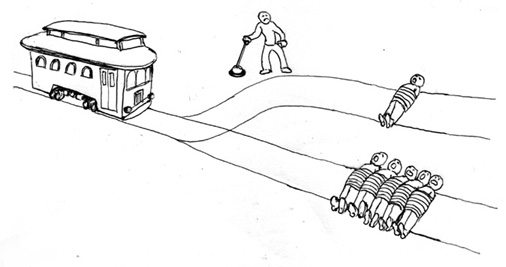
\includegraphics[width=0.6\textwidth]{trolley-example.jpg}
\end{center}

\wsprompt{Draw your own version of the trolley problem (you can change anything about the situation, as long as it is still a "trolley problem," broadly conceived). Use the back of this page if you want more space.}

\vspace{0.2\baselineskip}

\setlength{\fboxsep}{0pt}
\fbox{\parbox[c][3.6in][c]{\textwidth-2\fboxrule}{\hfill}}

\end{document}
